\section{Anhang}

\begin{table}[h]
	\begin{center}
		\def\arraystretch{1.4}
		\begin{tabular}{l | l | l}
			\textbf{Pilzart} & \textbf{Wissenschaftlicher Name} & \textbf{Essbarkeit}\\
			\hline
			Echter Pfifferling/Eierschwamm & Cantharellus cibarius & essbar\\
			Fichten-Reizker & Lactarius deterrimus & essbar\\
			Fichten-Steinpilz & Boletus edulis & essbar\\
			Flaschen-Stäubling & Lycoperdon perlatum & essbar\\
			Fliegenpilz & Amanita muscaria & giftig\\
			Frauen-Täubling & Russula cyanoxantha & essbar\\
			Gemeines Stockschwämmchen & Kuehneromyces mutabilis & essbar\\
			Grüner Knollenblätterpilz & Amanita phalloides & giftig\\
			Herbsttrompete/Totentrompete & Carterellus cornucopioides & essbar\\
			Körnchen-Röhrling & Suillus granulatus & essbar\\
			Maronen-Röhling & Xerocomus badius & essbar\\
			Nebelkappe/Nebelgrauer Trichterling & Clitocybe nebularis & giftig\\
			Perlpilz & Amanita rubescens & essbar\\
			Riesenschirmpilz/Parasolpilz & Macrolepiota procera & essbar\\
			Rötlicher Gallerttrichter & Tremiscus helvelloides & essbar\\
			Rotfuss-Röhrling & Xerocomus chrysenteron & essbar\\
			Schopf-Tintling & Coprinus comatus & essbar\\
			Hallimasch & Armillaria ostoyae & essbar\\
			Spitz-Morchel & Morchella conica & essbar\\
			Wiesen-Egerling/Wiesen-Champignon & Agaricus campestris & essbar\\
		\end{tabular}
	\end{center}
	\caption{Pilzarten}
	\label{table:shrooms}
\end{table}

\begin{table}[!htb]
	\def\arraystretch{1.4}
	\centering
	\begin{subtable}[t]{.5\linewidth}
		\begin{tabular}[t]{l | l }
			\multicolumn{2}{c}{\textbf{Netzaufbau}}\\
			\hline
			\textit{Layer}-Typ & Grösse\\
			\hline
			\hline
			Bildeingabe-\textit{Layer} & 200$\times$200$\times$3 \textit{oder}\\
			& 50$\times$50$\times$3 \textit{oder}\\
			& 10$\times$10$\times$3\\
			\hline
			
			\textit{Fully-ConnectedLayer}& 100 \textit{oder}\\
			& 60 \textit{oder}\\
			& 20\\
			\hline
			\textit{Output-Layer}& 21\\
		\end{tabular}
	\end{subtable}%
	\begin{subtable}[t]{.5\linewidth}
		\begin{tabular}[t]{l | l }
			\multicolumn{2}{c}{\textbf{Trainings-Einstellungen}}\\
			\hline
			\textit{Parameter} & Wert\\
			\hline
			\hline
			Lernrate $\eta$ & 0.001\\
			Mini-Batch-Grösse & 128\\
			Anz. Lernepochen & 7\\
			L2 Regularisierung & 0.0002\\
			Trainingsdaten mischen& nach Epoche\\
			\textit{Data-Augmentation}& - \\
		\end{tabular}
	\end{subtable} 
	\caption{\textit{Meta-Parameter} des Basis-\textit{SNN}s}
	\label{table:basic_snn_training}
\end{table}

\begin{table}[!htb]
	\def\arraystretch{1.4}
	\centering
	\begin{subtable}[t]{.5\linewidth}
		\begin{tabular}[t]{l | l }
			\multicolumn{2}{c}{\textbf{Netzaufbau}}\\
			\hline
			\textit{Layer}-Typ & Grösse\\
			\hline
			\hline
			Bildeingabe-\textit{Layer} & 200$\times$200$\times$3\\
			\hline
			\textit{Convolution-Layer}& Filter: 10 $\times$ 10\\
									  & Schrittweite: 4\\
									  & Anz. \textit{Feature Maps}: 20\\
			\hline
			\textit{max-Pooling-Layer}& Filter: 3 $\times$ 3\\
									  & Schrittweite: 2\\
			
			\hline
			\textit{Convolution-Layer}& Filter: 5 $\times$ 5\\
									  & Schrittweite: 1\\
									  & Anz. \textit{Feature Maps}: 40\\
			\hline
			\textit{max-Pooling-Layer}& Filter: 3 $\times$ 3\\
									  & Schrittweite: 2\\
			\hline
			\textit{Convolution-Layer}& Filter: 2 $\times$ 2\\
									  & Schrittweite: 1\\
									  & Anz. \textit{Feature Maps}: 60\\
			\hline
			\textit{max-Pooling-Layer}& Filter: 2 $\times$ 2\\
									  & Schrittweite: 2\\
			\hline
			\textit{Output-Layer}   & 21\\
		\end{tabular}
	\end{subtable}%
	\begin{subtable}[t]{.5\linewidth}
		\begin{tabular}[t]{l | l }
			\multicolumn{2}{c}{\textbf{Trainings-Einstellungen}}\\
			\hline
			\textit{Parameter} & Wert\\
			\hline
			\hline
			Lernrate $\eta$ & 0.001\\
			Mini-Batch-Grösse & 128\\
			Anz. Lernepochen & 20\\
			L2 Regularisierung & 0.0002\\
			Trainingsdaten mischen& nach Epoche\\
			\textit{Data-Augmentation}& - \\
		\end{tabular}
	\end{subtable} 
	\caption{\textit{Meta-Parameter} des Basis-\textit{CNN}s}
	\label{table:basic_cnn_training}
\end{table}


\begin{table}[!htb]
	\def\arraystretch{1.4}
	\centering
	\begin{subtable}[t]{.5\linewidth}
		\begin{tabular}[t]{l | l }
			\multicolumn{2}{c}{\textbf{Netzaufbau}}\\
			\hline
			\textit{Layer}-Typ \qquad\quad\quad& Grösse\\
			\hline
			\hline
			\multicolumn{2}{c}{\qquad\qquad\qquad\quad\textit{siehe Tabelle \ref{table:basic_cnn_training}}\qquad\qquad\qquad\qquad}\\
			\multicolumn{2}{c}{$\vdots$}\\
			\hline
		\end{tabular}
	\end{subtable}%
	\begin{subtable}[t]{.5\linewidth}
		\begin{tabular}[t]{l | l }
			\multicolumn{2}{c}{\textbf{Trainings-Einstellungen}}\\
			\hline
			\textit{Parameter} & Wert\\
			\hline
			\hline
			Lernrate $\eta$ & 0.001\\
			Mini-Batch-Grösse & 128\\
			Anz. Lernepochen & 20\\
			L2 Regularisierung & 0.0002\\
			Trainingsdaten mischen& nach Epoche\\
			\textit{Data-Augmentation}& Drehung: $\pm25^{\circ}$ \\
			& X-Versetzung: $\pm10px$ \\
			& Y-Versetzung: $\pm10px$ \\
			& X-Spiegelung: \checkmark \\
			& Y-Spiegelung: $\times$ \\
		\end{tabular}
	\end{subtable} 
	\caption{\textit{Meta-Parameter} des Basis-\textit{CNN}s mit \textit{Data-Augmentation}}
	\label{table:dataaug_training}
\end{table}



\begin{figure}[h]
	\centering
	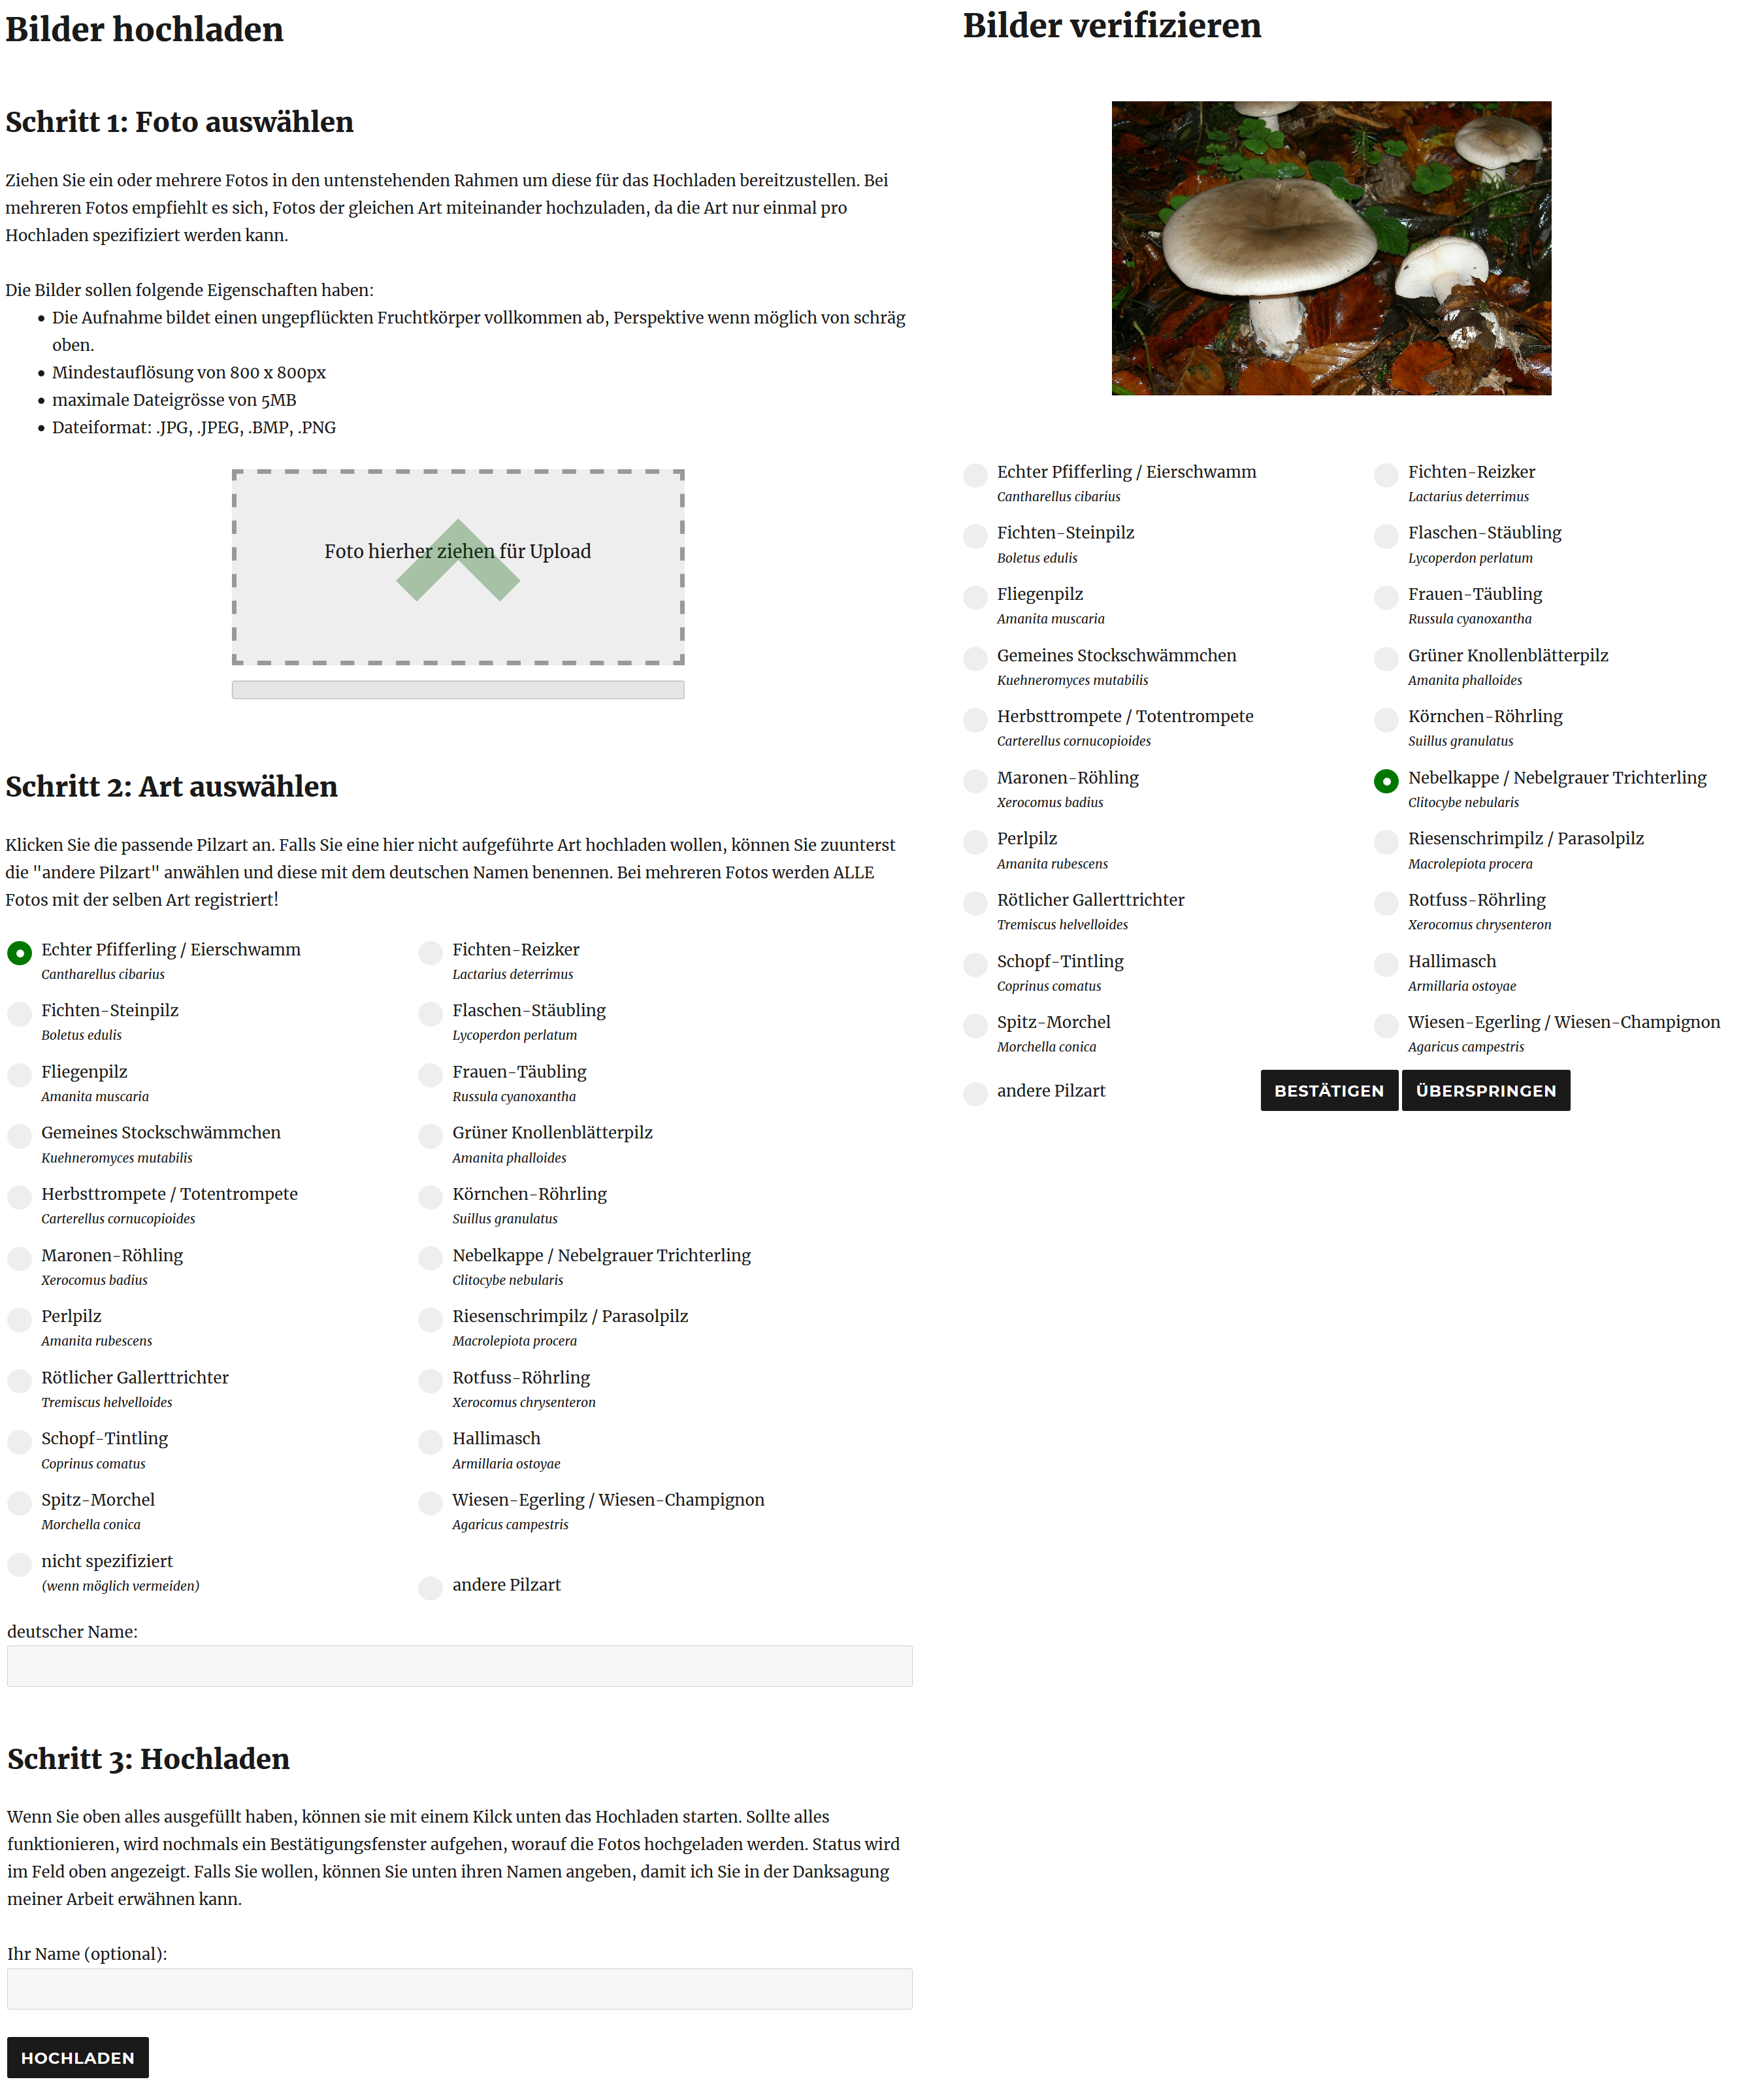
\includegraphics[width=\textwidth]{web_form}
	\caption[\textit{\textit{Hochladeformular \& Quiz}}]{Hochladeformular (links) und Quiz (rechts) von \textit{www.obermeier.ch}}
	\label{img:webpage}
\end{figure}